\documentclass[12pt, twoside]{article}
\usepackage{tikz}

\begin{document}
\begin{figure}
	\centering
	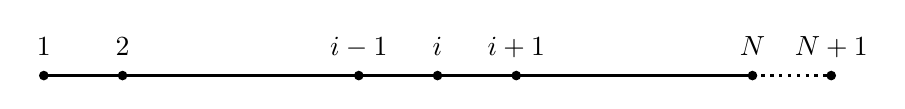
\begin{tikzpicture}[
			dot/.style = {circle,fill=black,inner sep=1pt, node contents={}},
			every node/.append style = {text depth=0.2ex}
		]
		\draw[very thick] (0,0) node (1)   [dot,label=$1$]  -- (1,0);
		\draw[very thick] (1,0) node (2)   [dot,label=$2$]  -- (2,0);
		\draw[very thick] (2,0) -- (4,0);
		\draw[very thick] (4,0) node (i-1) [dot,label=$i-1$] -- (5,0);
		\draw[very thick] (5,0) node (i)   [dot,label=$i$]   -- (6,0);
		\draw[very thick] (6,0) node (i+1) [dot,label=$i+1$] -- (7,0);
		\draw[very thick] (7,0) -- (9,0);
		\draw[dotted,very thick] (9,0)  node (N)   [dot,label=$N$] --
		(10,0) node (N+1) [dot,label=$N+1$];
	\end{tikzpicture}
	\caption{Visualization of meshing elements and intervals including the complex $N+1$ node}
	\label{fig:nodeline}
\end{figure}
\end{document}
